\documentclass[a4paper, 11pt]{article}
\usepackage{comment} % enables the use of multi-line comments (\ifx \fi) 
\usepackage{lipsum} %This package just generates Lorem Ipsum filler text. 
\usepackage{fullpage} % changes the margin
\usepackage{titlesec}
\usepackage{graphicx} 
\usepackage{caption} 

\graphicspath{ {./images/} }

\titlespacing\section{0pt}{12pt plus 4pt minus 2pt}{0pt plus 2pt minus 2pt}
\titlespacing\subsection{0pt}{12pt plus 4pt minus 2pt}{0pt plus 2pt minus 2pt}
\titlespacing\subsubsection{0pt}{12pt plus 4pt minus 2pt}{0pt plus 2pt minus 2pt}
                                   
\begin{document}
%Header-Make sure you update this information!!!!
\noindent
\large\textbf{19COC102 - Coursework} \hfill  
\normalsize Due on 16th March 2020, 12:00AM via Learn\hfill\\
\textbf{Peter Smith} \\
\hfill Student ID: B614743

\section*{Report A}% - Description of Tools, Methods, and changes made

After setting up a new Anaconda environment, Jupyter notebook and Tensorboard using the official documentation, I followed several tutorials and started experimenting. This involved modifying the model architectures, and trying different optimisers, loss functions, activation algorithms, and datasets. After completing both frameworks' tutorials, I felt more comfortable using Tensorflow.

\vspace{5mm} %5mm vertical space

I decided to keep my two architectures similar, as by comparing two similar neural networks (e.g. two networks with one key difference), it is easier to establish which elements of a model affect the results. This should lead to more accurate conclusions being drawn from the analysis.

For my architectures, I chose to use the model from the first tutorial I followed\cite{Tensorflow CNN Tutorial}. It is not complex, but it is a good starting point and allows us to add to it to see how the results change. For my second model, I have added Dropout layers to see the effect this has on overfitting. 

For my configurations, I wanted to see the differences using ReLU over TanH as a transfer function had on the result.
Initially I wanted to try more models (with added Normalisation) and more configurations (different learning rates), but I ran out of report space.

For my dataset, I chose CIFAR-10. It is a more difficult dataset to achieve a high accuracy in, and I thought this could provide greater differences in the performance of the neural networks. It is also the dataset I experimented with most and am most familiar with as a result.

\vspace{5mm} %5mm vertical space

Table \ref{tab:model details} shows the two model architectures I have chosen to investigate. All layers that are shared between the models also share the same parameter values. 

In Model 2, I have placed Dropout layers between Max Pooling and Convolutional Layers. This makes sense as it occurs after each 'core set' of 3 layers (Convolutional - Activation - Max Pooling).

\ifx In Model 3, I removed most of the convolutional, activation and pooling layers, leaving only the two fully-connected layers, separated by an Activation layer. This will give us contrast and show how adding convolutional layers impacts the accuracy of the network.\fi

\begin{table}[h]
\centering
\caption{Model Details}
\label{tab:model details}
\begin{tabular}{|l|l|l|}
\hline
      & Model 1 & Model 2  \\
\hline
Input & Convolution(32 parameters, (3,3) filter) & Convolution(32, (3,3))   \\
      & Activation & Activation   \\
      & Max Pooling((2,2) pool size) & Max Pooling((2,2))    \\
      &  & Dropout(0.25)   \\
      & Convolution(64 parameters, (3,3) filter) & Convolution(64, (3,3))   \\
      & Activation & Activation   \\
      & Max Pooling((2,2) pool size) & Max Pooling((2,2))    \\
      &  & Dropout(0.25)   \\
      & Convolution(64 parameters, (3,3) filter) & Convolution(64, (3,3))   \\
      & Activation & Activation   \\
      & Flatten & Flatten \\
      & Fully-Connected (Dense) (64 parameters)& Dense(64)  \\
      & Activation & Activation  \\
      &  & Dropout(0.5)   \\
Output & Dense(10 parameters) & Dense(10)  \\
\hline
\end{tabular}
\end{table}

\vspace{5mm} %5mm vertical space

The first layer in each network is also the 'Input Layer' and accepts the 'input shape' of the input data. For CIFAR-10, this is (32x32x3) because it is a 32 pixel by 32 pixel image in the 3 colour channels (Red, Green, Blue).

A Convolutional layer runs the data through the convolution operation, which processes it using a filter. The values within this filter are parameters that are changed throughout the training process to give more accurate classifications at the end. The size of this filter determines how much of an image is checked for a pattern.

The Activation layer introduces non-linearity to the data. This is usually done using ReLU but can also be done by softmax, sigmoid or tanh. It has other names, like transfer function, though Activation layer is what Tensorflow calls it. It allows for more combinations of layers. For example, two convolutional layers adjacent to one another do not make sense, as it is the same as having one, larger convolutional layer. With an activation function in between, their effectiveness is improved.

A Max Pooling layer looks through the data and, from each window, will only take the maximum value. This is a quick way to downsize the data into smaller pieces. The pool size specifies the degree of downsizing in the horizontal and vertical dimensions. This layer reduces the computational cost and allows future convolutional filters to check larger areas of the image.

The Dropout layer drops connections through the network randomly. This stops the network relying too much on any one parameter too heavily and can be used to counter overfitting. Overfitting is an error which occurs when the network learns to fit too closely to the test data, which leads to the network performing very well against the training data but not very well against any new, unfamiliar data. It often occurs when there are too many parameters, or insufficient data points. The Dropout layer drops some of these parameters and therefore can help counter this.

The Flatten function takes the data in matrix form and lines it up in a one-dimensional vector as a single-channel output. This is to format it for fully-connected layers.

Tensorflow calls fully-connected layers 'Dense' layers\cite{Dense}. In dense layers, every neuron is connected to every output. These often come at the end of the network. 

The output layer should be a dense layer. It should get all the features from the rest of the network and make decisions, mapping the vector it receives to the classes for classification. The final layer should only have \emph{n} parameters, where \emph{n} is the number of classes.

\subsection*{Configuration Details}
\ifx The 'learning rate' of a network is how much each parameter changes by in one run. If it is too high, the parameter can jump too far and it is difficult to achieve the 'true' value. The lower it is, the slower the network will take to learn, and will need more epochs. I will be using the 'Adam' optimiser as that is the recommended optimiser, however I will change its learning rate to test its effectiveness. One instance will have the default value (0.001) and the other instance will have 0.002, double the default value. \fi

TanH  (\(  \tanh (x) = \frac{ (e^x - e^{-x}) }{(e^x + e^{-x})}\)) and ReLU (\(  ReLU(x) = max(0,x)\)) are both Activation functions. They both introduce non-linearity, though there are different pros and cons to using either. In my configurations, when testing these, all instances of an Activation layer will be either ReLU or TanH.
\ifx
\begin{math}
\begin{minipage}{0.45\textwidth}
\[  \tanh (x) = \frac{ (e^x - e^{-x}) }{(e^x + e^{-x})}\]
\end{minipage}
\begin{minipage}{0.45\textwidth}
\[  ReLU(x) = max(0,x)\]
\end{minipage}
\end{math}
\fi
ReLU is faster, however it doesn't work for any negative numbers, while TanH does. ReLU only works for positive numbers, so if the input were huge positive numbers, they would stay huge (or get bigger), as no negative values could be applied \cite{CNN Lecture}.

These activation functions have been compared before, by Krizhevsky (2012), who found that 'networks with ReLU consistently learn several times faster than equivalents', and in his tests, ReLU reached a 25\% training error rate six times faster than a TanH equivalent \cite{Krizhevsky}.

\ifx I'm testing two different variables - the model changes and the activation function. These will predominantly be analysed independently - testing the activation function using the default Adam optimiser and testing the learning rate using the ReLU activation function.\fi

\section*{Report B}
\subsection*{Results}
When comparing two networks, I will be mainly looking at their validation accuracy and loss - the networks' accuracy/loss when presented with unfamiliar data. When looking at a single network, I will compare the training accuracy/loss with the validation accuracy/loss, as this can help identify overfitting.
For each case, I ran the network for 50 epochs. Accuracy is a percentage based on how many images can be correctly classified. Loss represents the error rate of a network - it uses a function to show how often a network makes incorrect guesses - this also takes into account partial guesses, such as a network guessing 55\% in favour of the correct answer, but 45\% in favour of an incorrect one. 

\subsubsection*{ReLU vs TanH}

\begin{figure}[h]
\begin{minipage}{0.45\textwidth}
\captionsetup{justification=centering}
\centering
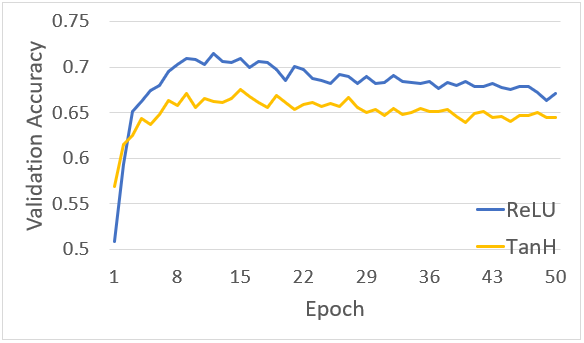
\includegraphics[scale=0.45]{1relucomp}
\caption[caption]{Model 1, \\ Accuracy of ReLU vs. TanH}
\label{m1a} % model 1 accuracy
\end{minipage}
\begin{minipage}{0.45\textwidth}
\captionsetup{justification=centering}
\centering
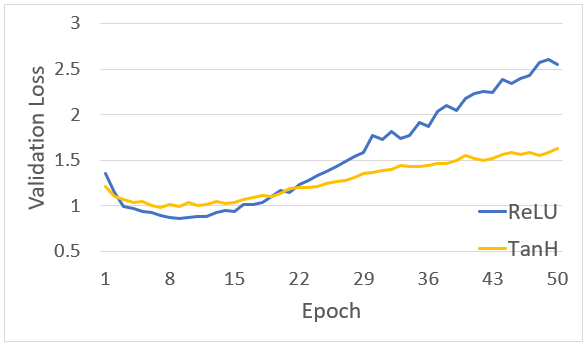
\includegraphics[scale=0.45]{1relucomploss}
\caption{Model 1,\\ Loss of ReLU vs. TanH}
\label{m1l}% model 1 loss
\end{minipage}
\end{figure}

As seen in Figure \ref{m1a}, the network that uses ReLU initially learns faster and maintains a higher accuracy throughout when compared to the network that uses TanH.

Figure \ref{m1l} shows that the ReLU case's loss initially falls faster than TanH. However both epochs reach a trough, before beginning to increase again. At this point, ReLU's loss increases at a greater rate than TanH's. A sign of overfitting is when the loss increases, as this shows the network is making more errors with unfamiliar data and is not improving.

\begin{figure}[h]
\begin{minipage}{0.45\textwidth}
\captionsetup{justification=centering}
\centering
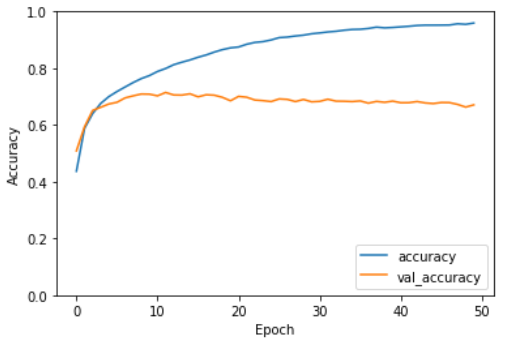
\includegraphics[scale=0.45]{1overfita}
\caption[caption]{Model 1, ReLU \\ Training Acc. vs. Validation Acc.}
\label{m1oa} % model 1 overfit accuracy
\end{minipage}
\begin{minipage}{0.45\textwidth}
\captionsetup{justification=centering}
\centering
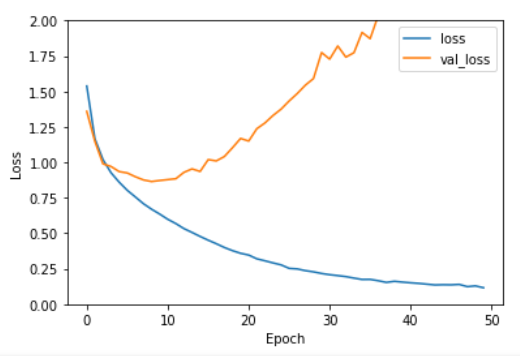
\includegraphics[scale=0.45]{1overfitl}
\caption{Model 1, ReLU\\ Training Loss vs. Validation Loss}
\label{m1ol}% model 1 overfit loss
\end{minipage}
\end{figure}

Another sign of overfitting is that the training accuracy continues to improve, but the validation accuracy gets worse or does not improve, as this shows the network is improving on the training data specifically and performs worse on the validation data. An increasing difference between the training and validation loss is another sign of overfitting. 

Using Figure \ref{m1oa}, we can see that very quickly the training accuracy and the validation accuracy (val\_accuracy) begin to diverge and the validation accuracy levels off quickly, whilst the training accuracy continues to increase. At the end, the two lines are significantly different. This is a clear sign of overfitting. Figure \ref{m1ol} shows the same, the two lines diverging at similar points. It could also be due to a too high learning rate, but that is not being measured.

\begin{figure}[h]
\begin{minipage}{0.45\textwidth}
\captionsetup{justification=centering}
\centering
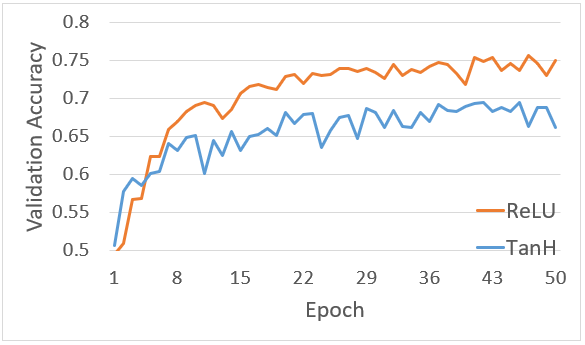
\includegraphics[scale=0.45]{2relucomp}
\caption[caption]{Model 2, \\ Accuracy of ReLU vs. TanH}
\label{m2a}
\end{minipage}
\begin{minipage}{0.45\textwidth}
\captionsetup{justification=centering}
\centering
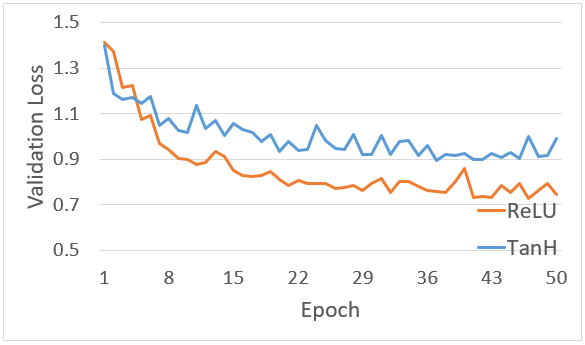
\includegraphics[scale=0.45]{2relucomploss}
\caption{Model 2,\\ Loss of ReLU vs. TanH}
\label{m2l}
\end{minipage}
\end{figure}

Model 2 has added Dropout layers, which are a counter-measure for overfitting. Where Model 1 suffered from a great deal of overfitting, I expected Model 2 to improve in that regard.

Figure \ref{m2a} shows that ReLU initially increases fast for longer than TanH, and stays at a higher accuracy throughout.

We see in Figure \ref{m2l} that neither loss increases, and we see a continuous decrease. This is better than Model 1 and is a good sign that no overfitting has occurred. ReLU also has a lower loss than TanH throughout most of the run.

\begin{figure}[h]
\begin{minipage}{0.45\textwidth}
\captionsetup{justification=centering}
\centering
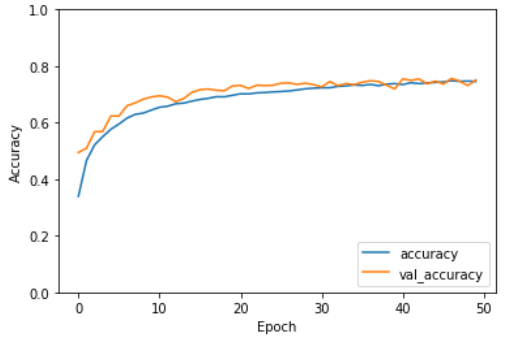
\includegraphics[scale=0.45]{2overfita}
\caption[caption]{Model 2, ReLU \\ Training Acc. vs. Validation Acc.}
\label{m2oa} % model 1 overfit accuracy
\end{minipage}
\begin{minipage}{0.45\textwidth}
\captionsetup{justification=centering}
\centering
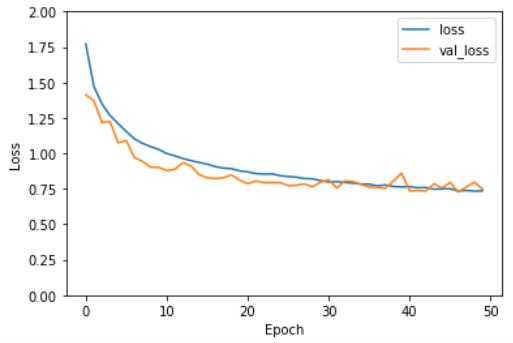
\includegraphics[scale=0.45]{2overfitl}
\caption{Model 2, ReLU\\ Training Loss vs. Validation Loss}
\label{m2ol}% model 1 overfit loss
\end{minipage}
\end{figure}

We see in both Figures \ref{m2oa} and \ref{m2ol} that the validation accuracy and loss keep close to the training lines throughout the run, showing no signs of overfitting. Both lines in Figure \ref{m2oa} continuously increase, however, it does increase quickly to begin with and then increases slower, which can be a sign that the learning rate is high, and maybe a lower learning rate at a later epoch, along with other fine-tuning could help improve this issue.
\subsubsection*{Model 1 vs. Model 2}

When comparing the models against each other, I'm only going to use the ReLU function, to save space in the report and as it seen as a superior function. The TanH networks had similar shapes, though the losses had different values.

\begin{figure}[h]
\begin{minipage}{0.45\textwidth}
\captionsetup{justification=centering}
\centering
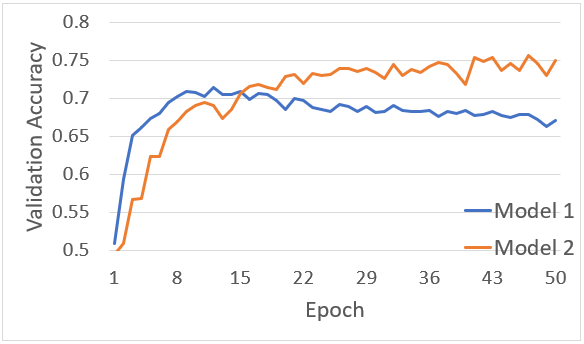
\includegraphics[scale=0.45]{12modelcomprelu}
\caption[caption]{\\ Accuracy of Model 1 vs. Model 2}
\label{m1m2ra}%model 1 model 2 relu accuracy
\end{minipage}
\begin{minipage}{0.45\textwidth}
\captionsetup{justification=centering}
\centering
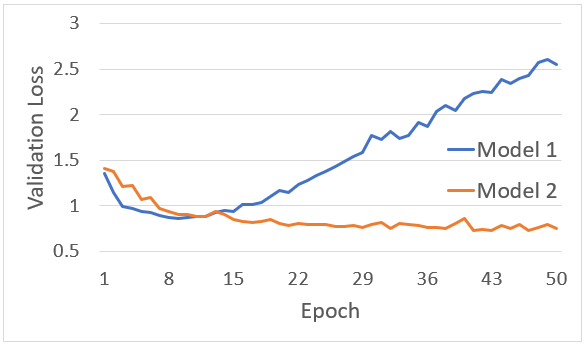
\includegraphics[scale=0.45]{12modelcompreluloss}
\caption{\\ Loss of Model 1 vs. Model 2}
\label{m1m2rl}%model 1 model 2 relu loss
\end{minipage}
\end{figure}

In Figure \ref{m1m2ra} we see that whilst Model 1 (without the dropout layers) climbs faster, it reaches a peak and starts decreasing slowly. Model 2 has a much 'healthier' shape - increasing at a fast rate, before slowly starting to level off, and then continuing to increase at a slower rate. Model 2 reaches a higher accuracy after 50 epochs, reaching 75\% accuracy compared to Model 1's 67\%. Some of this can be partialy explained by their Loss, as seen in Figure \ref{m1m2rl}. Model 1's accuracy slowly decreases when the loss begins to rise. The increased loss (error rate) - and the overfitting it represents - likely affects the accuracy of the network. In comparison, Model 2's loss decreases and then remains low. As Model 2 has not overfit, it is allowed to continue learning and as a result the accuracy continues to improve. 

\subsection*{Conclusion}

We have seen that ReLU leads to a network that learns faster than TanH. ReLU also tends to have a loss that falls faster and reaches a lower point than TanH.

In Model 1, we saw overfitting in both cases, and the ReLU network's loss increased at a greater rate than TanH. After 50 epochs, ReLU's loss was 2.5 whilst TanH's was only 1.5, which suggests that when overfitting, ReLU could be a worse function.
A reason why ReLU may struggle with overfitting is due to one of its disadvantages - it cannot handle any negative parameters as they become zero \cite{CNN Lecture}. This could lead to parameters getting bigger or staying large over time, when maybe they should get smaller.

Model 2 had Dropout layers, which are meant to help against overfitting and in both runs we did not see any sign of overfitting - their losses decreased and their accuracy increased consistently. In this, we saw ReLU climb faster for longer, reaching a higher accuracy. We also see ReLU's loss decrease faster for longer as well, reaching a lower loss than TanH. 
This suggests that when there is no overfitting, ReLU performs better in terms of both accuracy and loss. Due to the simplicity of the ReLU function, it is also fast to process. This did not have an effect on these tests as the dataset wasn't large enough for a significant time difference, but it is another benefit of ReLU. 

When comparing the two models, we see that Model 2 did not suffer from overfitting and reached a higher accuracy than Model 1 in both cases. The only difference between these models is added dropout layers, so I can be confident in saying that these layers were responsible for the lack of overfitting and the higher accuracy.

Adding Dropout layers is definitely helpful in the prevention of overfitting, and with overfitting countermeasures like this in place, ReLU is the superior function over TanH.

\begin{thebibliography}{9}

\bibitem{Tensorflow CNN Tutorial} Tensorflow 2020, \emph {Convolutional Neural Network (CNN)}, Tensorflow, last viewed 12 Mar 2020, (https://www.tensorflow.org/tutorials/images/cnn)

\bibitem{Dense} Tensorflow 2020, \emph{Custom layers}, Tensorflow, viewed 11 Mar 2020, (https://www.tensorflow.org/tutorials/customization/custom\_layers).

\bibitem{Krizhevsky} Krizhevsky, A; Sutskever, I; Hinton, G. 2012, 'ImageNet Classification with Deep Convolutional Neural Networks', \emph{In NIPS 2012}, viewed 11 Mar 2020 (http://papers.nips.cc/paper/4824-imagenet-classification-with-deep-convolutional-neural-networks.pdf).

\bibitem{CNN Lecture} Soltoggio, A 2020, \emph{Deep Convolutional Neural Networks (CNNs)}, lecture notes, Advanced AI Systems 19COC102, Loughborough University, delivered 25th Feb 2020.

\end{thebibliography}

\end{document}
